\section{سناریوهای کوئری و خط پایه}
\label{sec:scenarios}

\subsection{هشت سناریوی گزارش}

طبق سند پروژه، هشت کوئری تحلیلی روی داده تعریف و در فایل \Rl{sql/04_scenarios.sql} نوشته شده‌اند. جدول \ref{tab:scenarios} خلاصه‌ی آن‌هاست؛ همه از \lr{CROSS JOIN LATERAL unnest(...)} برای باز کردن ستون‌های آرایه‌ای (\lr{genres}، \lr{directors}) استفاده می‌کنند.

\begin{table}[h]
\centering
\caption{هشت سناریوی کوئری گزارش}
\label{tab:scenarios}
\begin{tabular}{@{}p{0.7cm}p{6cm}p{7.3cm}@{}}
\toprule
\textbf{\#} & \textbf{عنوان} & \textbf{ویژگی اصلی} \\
\midrule
\lr{1} & میانگین امتیاز فیلم به تفکیک ژانر & \lr{unnest(genres)}، پیوند با \lr{title\_ratings} \\
\lr{2} & \lr{10} فیلم برتر بر اساس تعداد رأی (حداقل \lr{1000} رأی) & \lr{ORDER BY num\_votes DESC LIMIT 10} \\
\lr{3} & \lr{20} کارگردان برتر بر اساس تعداد فیلم و میانگین امتیاز & \lr{unnest(directors)}، \lr{LEFT JOIN} به امتیازها \\
\lr{4} & میانگین امتیاز سالانه از سال \lr{2000} به بعد & فیلتر بازه‌ای روی \lr{start\_year} \\
\lr{5} & بازیگرانی با بیش از \lr{5} ژانر متفاوت & سنگین‌ترین کوئری؛ از \lr{title\_principals} (\lr{~90M} سطر) شروع می‌شود \\
\lr{6} & سریال‌هایی با بیشترین تعداد فصل & پیوند \lr{title\_episode} به والد از طریق \lr{parent\_tconst} \\
\lr{7} & پرتکرارترین جفت ژانر هم‌زمان & خودپیوندِ دو \lr{unnest} با \lr{g1.genre < g2.genre} \\
\lr{8} & \lr{5} فیلم بلندتر در هر ژانر & تابع پنجره‌ای \lr{ROW\_NUMBER() OVER (PARTITION BY genre ...)} \\
\bottomrule
\end{tabular}
\end{table}

برای نمونه، سناریوی \lr{1} (که خود سند پروژه هم آن را مثال زده) این‌طور است:

\begin{latin}
\begin{lstlisting}[language=SQL, caption={Scenario 1: average rating by genre}]
SELECT g.genre,
       ROUND(AVG(tr.average_rating), 2) AS avg_rating,
       COUNT(*)                         AS rated_titles
FROM   imdb.title_basics tb
CROSS  JOIN LATERAL unnest(tb.genres) AS g(genre)
JOIN   imdb.title_ratings tr ON tr.tconst = tb.tconst
WHERE  tb.title_type = 'movie'
GROUP  BY g.genre
ORDER  BY AVG(tr.average_rating) DESC;
\end{lstlisting}
\end{latin}

\subsection{رفتار مورد انتظار در خط پایه}

قبل از هر ایندکس‌گذاری (بخش \ref{sec:indexing})، فقط کلیدهای اصلی ایندکس دارند. این یعنی:

\begin{itemize}
\item \textbf{اسکن ترتیبی همه‌جا.} چون شرط‌هایی مثل \lr{title\_type = 'movie'} یا \lr{num\_votes >= 1000} هیچ ایندکسی ندارند، برنامه‌ریز مجبور است کل جدول را بخواند و سطر به سطر فیلتر کند. روی جدول‌های بزرگ (\lr{title\_basics} حدود \lr{12} میلیون سطر، \lr{title\_principals} حدود \lr{90} میلیون سطر)، این به‌صورت \lr{Parallel Seq Scan} دیده می‌شود.
\item \textbf{پیوند درهم (\lr{Hash Join}) با ریزش روی دیسک.} چون \lr{work\_mem} سراسری روی \lr{32MB} نگه داشته شده، اگر جدول هش یک پیوند از این مقدار بزرگ‌تر شود، به چند \lr{batch} روی دیسک می‌شکند.
\item \textbf{تجمیع و مرتب‌سازی ریزشی.} \lr{HashAggregate} و \lr{Sort} هم وقتی از \lr{work\_mem} بزرگ‌تر شوند، روی دیسک ریزش می‌کنند.
\item \textbf{از نظر طراحی، سناریوی \lr{5} باید سنگین‌ترین باشد.} این سناریو از \lr{title\_principals} شروع می‌شود که به‌طور طبیعی بزرگ‌ترین جدول این پروژه است (نزدیک \lr{90} میلیون سطر). بعد به \lr{title\_basics} و \lr{name\_basics} پیوند می‌خورد، ژانرها باز می‌شوند، و در آخر \lr{COUNT(DISTINCT genre)} گرفته می‌شود. پس انتظار داریم این کوئری بیشترین فایل موقت و بیشترین زمان را در خط پایه داشته باشد. اما در اجرای واقعی این پروژه، \lr{title\_principals} به‌خاطر محدودیت فضای دیسک فقط با \lr{8} میلیون سطر (حدود \lr{9\%} حجم واقعی) بارگذاری شد (جزئیات در بخش \ref{sec:real-data-scale})؛ درعوض \lr{title\_crew} و \lr{name\_basics} کامل ماندند. به همین دلیل سناریوی \lr{3} -- که از این دو جدول کامل می‌خواند -- در عمل سنگین‌تر از سناریوی \lr{5} از آب درآمد. این خودش یک نمونه‌ی خوب است: همیشه باید با عدد واقعی سنجید، نه فقط با اندازه‌ی نظری جدول.
\end{itemize}

قبل از اندازه‌گیری خط پایه، دستور \lr{ANALYZE} روی هر هفت جدول اجرا می‌شود. بلافاصله بعد از یک بارگذاری انبوه، آمار برنامه‌ریز خالی است (\lr{reltuples = -1})؛ بدون این آمار، برنامه‌ریز اندازه‌ی پیوندها را الکی حدس می‌زند و پلن‌های خیلی بد و غیرقابل‌تکرار انتخاب می‌کند. اجرای \lr{ANALYZE} این آمار را تازه می‌کند تا عدد «قبل از بهینه‌سازی» معنا داشته باشد.

اجرای این اندازه‌گیری‌ها با \Rl{scripts/run_scenarios.py} خودکار شده است: این اسکریپت \lr{ANALYZE} را اجرا می‌کند، برای هر سناریو خروجی \lr{EXPLAIN (ANALYZE, BUFFERS, SETTINGS)} را در \Rl{results/explain/} می‌نویسد، و زمان اجرا را در \Rl{results/timings/scenario_timings.csv} ثبت می‌کند.

شکل \ref{fig:success} یک اجرای واقعی و موفق را نشان می‌دهد: هر دو کانتینر \lr{Docker} در حال اجرا هستند، و سناریوی \lr{2} با ایندکس واقعی \lr{idx\_title\_ratings\_votes\_desc} به‌جای \lr{Seq Scan} از \lr{Index Scan} استفاده می‌کند.

\begin{figure}[h]
\centering
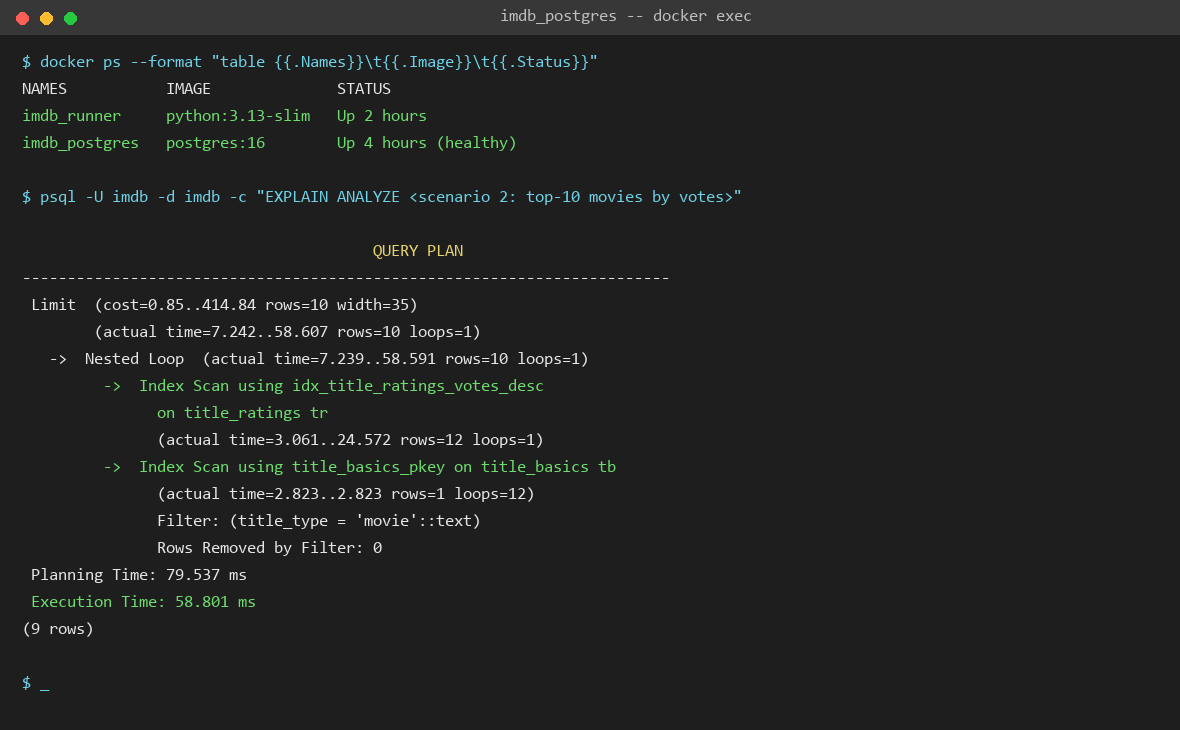
\includegraphics[width=0.85\linewidth]{figures/successful_execution.png}
\caption{اجرای موفق: کانتینرهای \lr{Docker} در حال کار، و \lr{EXPLAIN ANALYZE} واقعی سناریوی \lr{2} بعد از ایندکس‌گذاری}
\label{fig:success}
\end{figure}
